% chapters/planning.tex — Planning chapter (narrative text only)
\chapter{Planning and Task Decomposition}
\label{chap:planning}

Planning is the capacity of an agent to decompose a high-level goal into a
sequence of achievable sub-tasks and to select actions that advance toward
that goal~\cite{correa2025planningperformance}.
Frontier \LLM{}s have shown remarkable improvements in planning by leveraging
chain-of-thought reasoning and search-based exploration.
\index{planning}
\index{task decomposition}

% Nomenclature entries — FR-26: ≥2 symbols required
\nomenclature{$\AgentSet$}{Set of agents in a multi-agent system}
\nomenclature{$\StateSpace$}{State space of the planning environment}
\nomenclature{$\Policy$}{Policy mapping observations to action distributions}
\nomenclature{$\ValueFn$}{Value function estimating cumulative expected reward}

\section{Formal Objective}
\label{sec:planning-objective}

Let $\AgentSet$ denote the set of agents operating in a state space
$\StateSpace$ with action space $\ActionSpace$.
A policy $\Policy : \StateSpace \to \ActionSpace$ induces a trajectory
$\tau = (s_0, a_0, s_1, a_1, \ldots, s_T)$.
The planning objective is to find the policy that maximises cumulative reward:

\begin{equation}
  \label{eq:planning-objective}
  \Policy^{*} = \argmax_{\Policy} \;\E\!\left[\sum_{t=0}^{T} \gamma^{t}\,
  \Reward(s_t, a_t)\right]
\end{equation}

where $\gamma \in (0,1]$ is a discount factor and $\Reward$ is the scalar
reward received at each step.
As expressed in Equation~\eqref{eq:planning-objective}, the agent must
balance immediate and future rewards — a challenge that hierarchical
decomposition addresses by reducing the effective horizon.

\begin{definition}[Hierarchical Task Decomposition]
  \label{def:htd}
  A \emph{hierarchical task decomposition} of goal $g$ is a tree of
  sub-goals $\{g_1, \ldots, g_k\}$ such that, for any state in which all
  $g_i$ have been achieved, the agent has also achieved $g$.
\end{definition}

\section{Benchmark Evidence}
\label{sec:planning-benchmarks}

\cite{correa2025planningperformance} evaluated frontier \LLM{}s on classical
planning benchmarks (Blocksworld, ALFWorld, GSM8K) and found that
search-augmented models outperform pure chain-of-thought by a significant
margin.
Table~\ref{tab:planning-methods} summarises the key results.

% tables/planning_methods.tex — Standalone table: planning method comparison.
% Included from chapters/planning.tex via % tables/planning_methods.tex — Standalone table: planning method comparison.
% Included from chapters/planning.tex via % tables/planning_methods.tex — Standalone table: planning method comparison.
% Included from chapters/planning.tex via \input{tables/planning_methods.tex}
% inside a table environment.
\begin{table}[ht]
  \centering
  \caption{Comparison of planning approaches in frontier \LLM agents.}
  \label{tab:planning-methods}
  \begin{tabular}{@{}llcc@{}}
    \toprule
    \textbf{Method} & \textbf{Strategy} & \textbf{Benchmark} & \textbf{Score} \\
    \midrule
    GPT-4o          & Chain-of-thought  & Blocksworld        & 74\%           \\
    o1-preview      & Search + backtrack & Blocksworld       & 81\%           \\
    Claude 3.5      & ReAct             & ALFWorld           & 67\%           \\
    Gemini 1.5 Pro  & Tree-of-thought   & GSM8K              & 95\%           \\
    \bottomrule
  \end{tabular}
  \smallskip

  \footnotesize Scores from \cite{correa2025planningperformance}.
  Higher is better; benchmarks are not directly comparable across rows.
\end{table}

% inside a table environment.
\begin{table}[ht]
  \centering
  \caption{Comparison of planning approaches in frontier \LLM agents.}
  \label{tab:planning-methods}
  \begin{tabular}{@{}llcc@{}}
    \toprule
    \textbf{Method} & \textbf{Strategy} & \textbf{Benchmark} & \textbf{Score} \\
    \midrule
    GPT-4o          & Chain-of-thought  & Blocksworld        & 74\%           \\
    o1-preview      & Search + backtrack & Blocksworld       & 81\%           \\
    Claude 3.5      & ReAct             & ALFWorld           & 67\%           \\
    Gemini 1.5 Pro  & Tree-of-thought   & GSM8K              & 95\%           \\
    \bottomrule
  \end{tabular}
  \smallskip

  \footnotesize Scores from \cite{correa2025planningperformance}.
  Higher is better; benchmarks are not directly comparable across rows.
\end{table}

% inside a table environment.
\begin{table}[ht]
  \centering
  \caption{Comparison of planning approaches in frontier \LLM agents.}
  \label{tab:planning-methods}
  \begin{tabular}{@{}llcc@{}}
    \toprule
    \textbf{Method} & \textbf{Strategy} & \textbf{Benchmark} & \textbf{Score} \\
    \midrule
    GPT-4o          & Chain-of-thought  & Blocksworld        & 74\%           \\
    o1-preview      & Search + backtrack & Blocksworld       & 81\%           \\
    Claude 3.5      & ReAct             & ALFWorld           & 67\%           \\
    Gemini 1.5 Pro  & Tree-of-thought   & GSM8K              & 95\%           \\
    \bottomrule
  \end{tabular}
  \smallskip

  \footnotesize Scores from \cite{correa2025planningperformance}.
  Higher is better; benchmarks are not directly comparable across rows.
\end{table}


\section{The Agentic Perception--Action Loop}
\label{sec:planning-loop}

Figure~\ref{fig:agent-loop} illustrates the core agentic loop in which an
agent repeatedly observes its environment, reasons about the next action,
and executes that action.

\begin{figure}[ht]
  \centering
  % figures/agent_loop.tex — TikZ diagram of the agentic perception-action loop.
% Included from a chapter via % figures/agent_loop.tex — TikZ diagram of the agentic perception-action loop.
% Included from a chapter via % figures/agent_loop.tex — TikZ diagram of the agentic perception-action loop.
% Included from a chapter via \input{figures/agent_loop.tex} inside a
% figure environment.  All paths are relative to the compilation root.
\begin{tikzpicture}[
  node distance=2.8cm and 2.2cm,
  box/.style={
    rectangle, draw=blue!60, fill=blue!8, rounded corners=4pt,
    minimum width=2.6cm, minimum height=1.0cm, text centered,
    font=\small\sffamily
  },
  env/.style={
    ellipse, draw=green!50!black, fill=green!10,
    minimum width=3.0cm, minimum height=1.0cm, text centered,
    font=\small\sffamily
  },
  arr/.style={-{Stealth[scale=1.1]}, thick, draw=gray!70}
]
  \node[box] (observe) {Observe};
  \node[box, right=of observe] (reason) {Reason};
  \node[box, right=of reason] (act) {Act};
  \node[env, below=1.8cm of reason] (env) {Environment};

  \draw[arr] (observe) -- (reason);
  \draw[arr] (reason) -- (act);
  \draw[arr] (act) -- ++(0,-1.2) -| (env);
  \draw[arr] (env) -- ++(-4.2,0) |- (observe);
\end{tikzpicture}
 inside a
% figure environment.  All paths are relative to the compilation root.
\begin{tikzpicture}[
  node distance=2.8cm and 2.2cm,
  box/.style={
    rectangle, draw=blue!60, fill=blue!8, rounded corners=4pt,
    minimum width=2.6cm, minimum height=1.0cm, text centered,
    font=\small\sffamily
  },
  env/.style={
    ellipse, draw=green!50!black, fill=green!10,
    minimum width=3.0cm, minimum height=1.0cm, text centered,
    font=\small\sffamily
  },
  arr/.style={-{Stealth[scale=1.1]}, thick, draw=gray!70}
]
  \node[box] (observe) {Observe};
  \node[box, right=of observe] (reason) {Reason};
  \node[box, right=of reason] (act) {Act};
  \node[env, below=1.8cm of reason] (env) {Environment};

  \draw[arr] (observe) -- (reason);
  \draw[arr] (reason) -- (act);
  \draw[arr] (act) -- ++(0,-1.2) -| (env);
  \draw[arr] (env) -- ++(-4.2,0) |- (observe);
\end{tikzpicture}
 inside a
% figure environment.  All paths are relative to the compilation root.
\begin{tikzpicture}[
  node distance=2.8cm and 2.2cm,
  box/.style={
    rectangle, draw=blue!60, fill=blue!8, rounded corners=4pt,
    minimum width=2.6cm, minimum height=1.0cm, text centered,
    font=\small\sffamily
  },
  env/.style={
    ellipse, draw=green!50!black, fill=green!10,
    minimum width=3.0cm, minimum height=1.0cm, text centered,
    font=\small\sffamily
  },
  arr/.style={-{Stealth[scale=1.1]}, thick, draw=gray!70}
]
  \node[box] (observe) {Observe};
  \node[box, right=of observe] (reason) {Reason};
  \node[box, right=of reason] (act) {Act};
  \node[env, below=1.8cm of reason] (env) {Environment};

  \draw[arr] (observe) -- (reason);
  \draw[arr] (reason) -- (act);
  \draw[arr] (act) -- ++(0,-1.2) -| (env);
  \draw[arr] (env) -- ++(-4.2,0) |- (observe);
\end{tikzpicture}

  \caption{The agentic perception--action loop.  Arrows show the cyclic flow:
    the agent \emph{observes} state, \emph{reasons} to select an action, and
    \emph{acts} on the environment, which transitions to a new state.}
  \label{fig:agent-loop}
\end{figure}

\section{Graph: Planning Benchmark Comparison}
\label{sec:planning-graph}

Figure~\ref{fig:planning-benchmark} shows the planning benchmark comparison
generated by the Phase~8 graph pipeline (P8-I01).

\begin{figure}[ht]
  \centering
  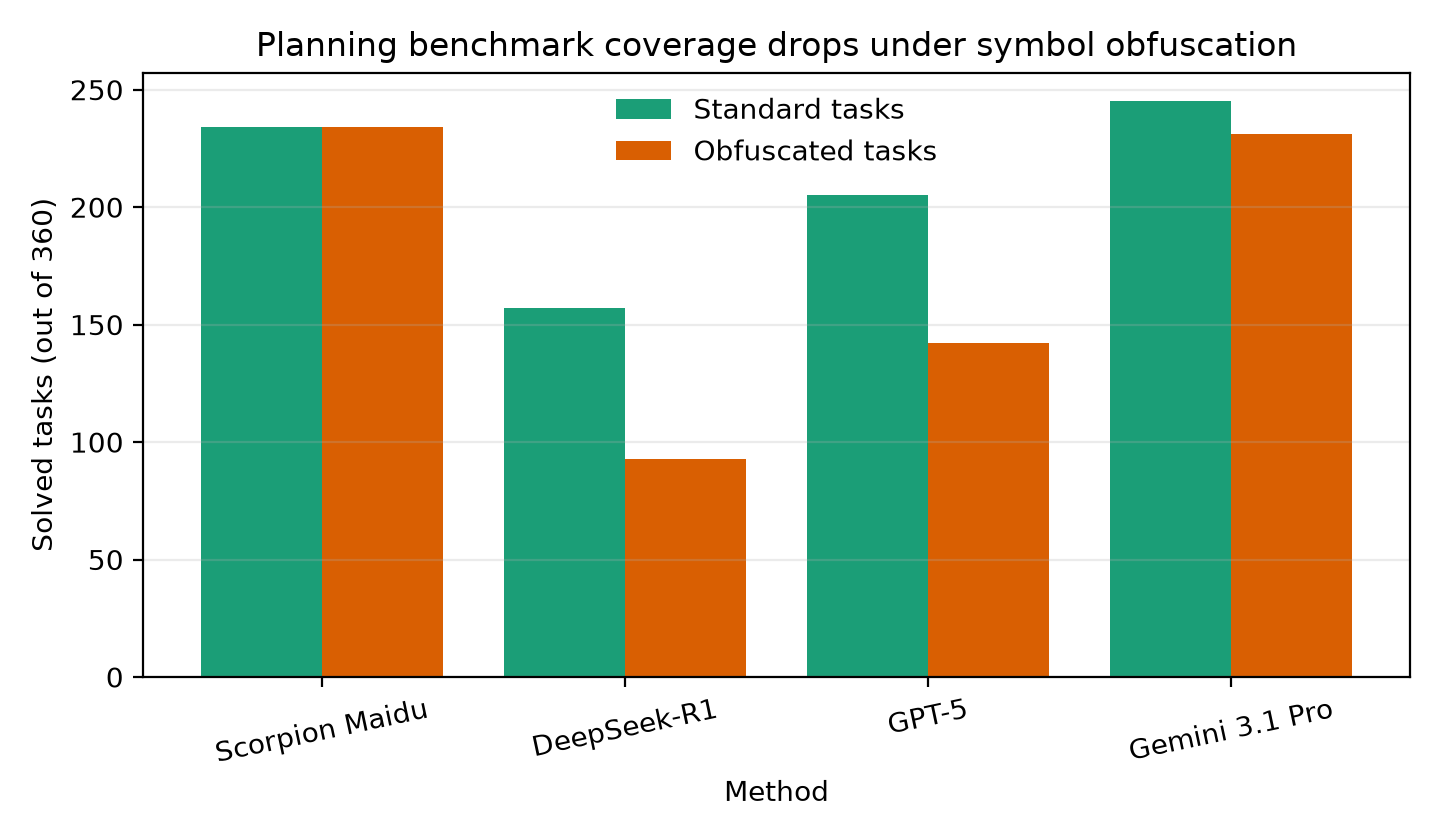
\includegraphics[width=0.85\linewidth]{figures/planning_benchmark_comparison_02e65860}
  \caption{Planning benchmark comparison across frontier \LLM{}s.
    Generated deterministically by the Phase~8 visualisation pipeline.}
  \label{fig:planning-benchmark}
\end{figure}
